\documentclass{article}
\usepackage[utf8]{inputenc}
\usepackage[greek,english]{babel}
\usepackage{alphabeta}
\usepackage{graphicx}
\usepackage{hyperref} 
\usepackage{listings}
\usepackage{subcaption}
\usepackage{mathtools}
\usepackage{tikz}
\usepackage{multirow}
\date{}

















\begin{document}

\begin{titlepage} % Suppresses displaying the page number on the title page and the subsequent page counts as page 1
	
	\raggedleft % Right align the title page
	
	\rule{1pt}{\textheight} % Vertical line
	\hspace{0.05\textwidth} % Whitespace between the vertical line and title page text
	\parbox[b]{0.75\textwidth}{ % Paragraph box for holding the title page text, adjust the width to move the title page left or right on the page
		
		{\Huge\bfseries Προσομοίωση \\ \\
		και Μοντελοποίηση\\ \\ Συστημάτων}\\[2\baselineskip] % Title
		{\large\textit{ }}\\[4\baselineskip] % Subtitle or further description
		{\Large\textsc{Ιωάννης-Παναγιώτης \\Μπουντουρίδης}} %
	\\	\\{\large\textsc{ΑΕΜ: 8872}} % Author name, lower case for consistent small caps
		
		\vspace{0.5\textheight} % Whitespace between the title block and the publisher
		
		{\noindent \textit{project}}\\[\baselineskip] % Publisher and logo
	}

\end{titlepage}
\newpage
\section*{1) Γραμμικό σύστημα}
\large
Δοθέντος του παρακάτω συστήματος:
\begin{center}

 \begin{tikzpicture}[scale=1]
\draw (0,0) node[rectangle,inner sep=18pt,draw] (s) {Σύστημα};
\draw[->] (s.east) -- ++(1,0) node[right] {$y(t)$};
\draw[<-] (s.west) -- ++(-1,0) node[left] {$u(t)$};

\draw[->,black] (s) ++(0.2,-2) node[below] {Νόμος $T$} to[bend left] (s);
\end{tikzpicture}
\end{center}
έστω οι έξοδοι 
\begin{equation*}
y_1(t) = T\left[u_1(t)\right]
\end{equation*}
\begin{equation*}
y_2(t) = T\left[u_2(t)\right]
\end{equation*}
το σύστημα είναι γραμμικό ανν: 
\begin{equation*}
T\left[u_1(t) + u_2(t)\right] = T\left[u_1(t)\right] + T\left[u_2(t)\right]
\end{equation*}
επιλέγουμε τις εισόδους: 
\begin{equation*}
\boxed{
u_1 = 4 \cdot sin(2 \cdot t)
}
\end{equation*}
\begin{equation*}
\boxed{
u_2 = 3 \cdot cos(5 \cdot t)
}
\end{equation*}
\begin{equation*}
\boxed{
u = 4 \cdot sin(2 \cdot t) + 3 \cdot cos(5 \cdot t) = u_1 + u_2
}
\end{equation*}
παίρνουμε τις εξόδους απο το αρχείο \textit{out.p}:
\begin{equation*}
\boxed{
y_1(t) = T\left[u_1(t)\right]
}
\end{equation*}
\begin{equation*}
\boxed{
y_1(t) = T\left[u_2(t)\right]
}
\end{equation*}
\begin{equation*}
\boxed{
y(t) = T\left[u(t)\right] = T\left[u_1(t) + u_2(t)\right]
}
\end{equation*}
ορίζουμε ως σφάλμα την διαφορά εξόδου των σημάτων:
\begin{equation*}
e(t) = y(t) - y_1(t) -y_2(t)
\end{equation*}
για χρόνο:  $ 0 \leq t \leq 20 \enspace$   με βήμα 0.001 sec παρουσιάζεται το σφάλμα τιμών συναρτήσει του χρόνου.
\newpage
\section*{Γραφική παράσταση σφάλματος}
 \begin{figure*}[h!]
\centering
 	\advance\leftskip-7.5cm
  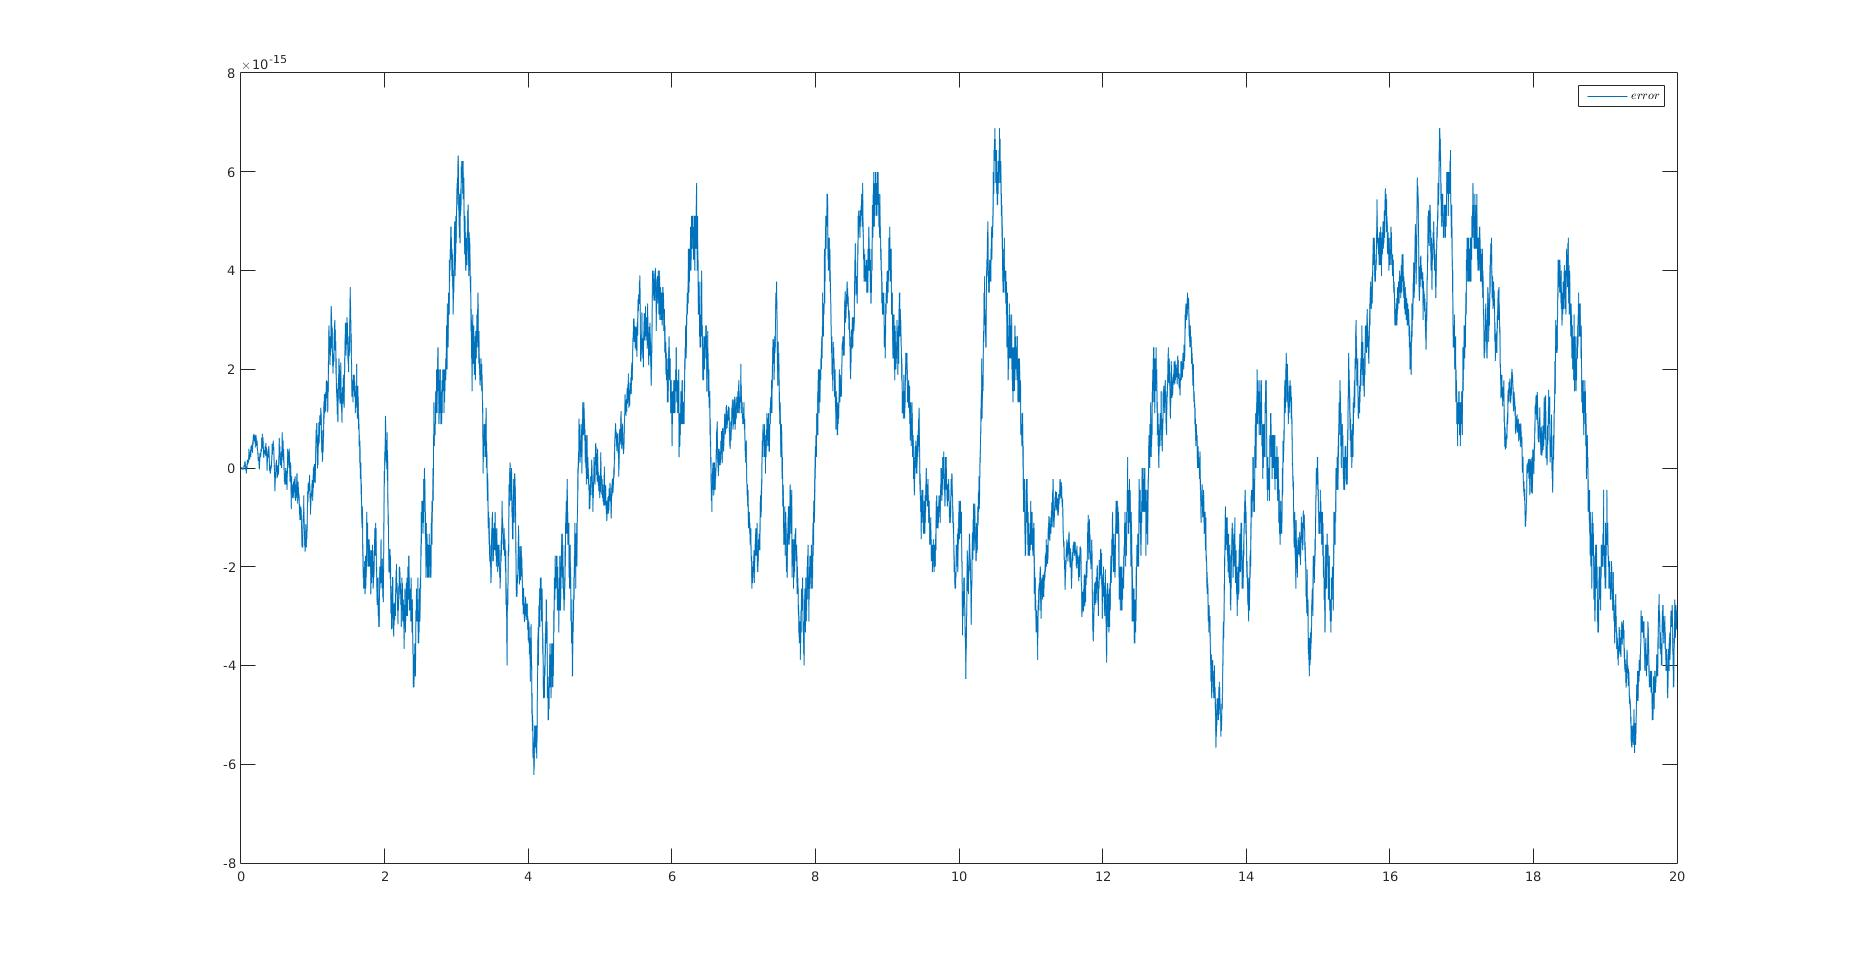
\includegraphics[width=265mm,scale=2]{assets/error.jpg}
\end{figure*}Το σφάλμα της γραφικής παράστασης είναι της κλίμακας $10^{-15}$ και θεωρείται αμεληταίο. Είναι σαφές λοιπόν πως ικανοποιείται ορισμός του \textbf{γραμμικού συστήματος.}
\begin{equation*}
\boxed{
T\left[u_1(t) + u_2(t)\right] = T\left[u_1(t)\right] + T\left[u_2(t)\right]
}
\end{equation*}
Ο κώδικας για την υλοποίηση του έλεγχου γραμμικότητας του συστήματος είναι διαθέσιμος στο αρχείο \textit{check\_linear.m} εντος του φάκελου  \textit{matlab\_source\_code}
 
\clearpage
\Large
\section*{Μέθοδος μη-πραγματικού χρόνου}

\par
 Για την εκτίμηση των παραμέτρων με μια μέθοδο μη-πραγματικού χρόνου, \textbf{επιλέγουμε τον αλγόριθμο των ελαχίστων τετραγώνων.} \par
Επειδή οι τάξεις της εισόδου και της εξόδου του συστήματος μας είναι παντελώς άγνωστες, έστω n και m αντίστοιχα οι τάξεις της εισόδου και της εξόδου που επιθυμούμε να βρούμε.
\par Το σύστημα στο οποίο αναζητούμε τις λύσεις των παραμέτρων θα είναι της μορφής
\begin{equation*}
\hspace*{-2.5cm} 
y^{(n)} + θ_0 \cdot y^{(n-1)} + θ_1 \cdot  y^{(n-2)} + ... + θ_{n-1} \cdot  y =  θ_n \cdot u^{(m)} + θ_{n+1} \cdot u^{(m-1)} + θ_{n+2} \cdot u^{(m-2)} + ... +  θ_{n+m} \cdot u 
\end{equation*}
επιθυμούμε να φέρουμε το σύστημα στην μορφή
\begin{equation*}
y = {θ_λ}^{\!T}ζ
\end{equation*}
οπου 
\begin{equation*}
{θ_λ} = \begin{bmatrix}
    {{θ_1}^*}^{\!T} - {λ}^{\!T} & {{θ_2}^*}^{\!T}   
     
  \end{bmatrix}^{\!T}
\end{equation*}
\[
{θ_1}^* = \begin{bmatrix}
    θ_0 & θ_1 & θ_2 & ... & θ_{n-1}  
     
  \end{bmatrix}^{\!T}
\]
\[
{θ_2}^* = \begin{bmatrix}
    θ_{n} & θ_{n+1} & θ_{n+2} & ... & θ_{n+m}   
     
  \end{bmatrix}^{\!T}
\]
και για κάθε περίπτωση επιλέγουμε ενα φίλτρο n ταξής
\begin{equation*}
Λ(s) = s^n + λ^{Τ} Δ_{n-1}
\end{equation*}
\begin{equation*}
λ = [\enspace λ_1 \enspace λ_2 \enspace ... \enspace λ_n \enspace ] ^{Τ}
\end{equation*}
κατα τα γνωστά συμφωνα με την θεωρία
\begin{equation*}
ζ = \begin{bmatrix}
-\frac{{Δ^{Τ}}_{n-1}(s)}{Λ(s)}  y & \frac{{Δ^{Τ}}_{m}(s)}{Λ(s)}u  
\end{bmatrix}
\end{equation*}

Συνεπώς αυτό που απαιτείται στην μοντελοποίηση ενος συστήματος κατα μαύρο κουτί είναι να υποθέσουμε τις άγνωστες τάξεις εισόδου και εξόδου.
\clearpage
\Large {}
Παρακάτω παρουσιάζεται μια σειρά δοκιμών που έγινε για την επιλογή της τάξης εισόδου και εξόδου του συστήματος.
\par Αμέσως μετά την απεικόνιση των διαγραμμάτων που θα ακολουθήσουν κρίνουμε κατα πόσο εγκυρα ηταν αποτελέσματα κάθε μοντελου. 
\begin{center}
\begin{tabular}{ |c|c|c| } 
 \hline
$\qquad$ $\qquad$ Δοκιμές $\qquad$ $\qquad$ &$\qquad$ n $\qquad$& $\qquad$ m $\qquad$ \\ 
  \hline
 $1^{η}$ δοκιμή & 1 & 0 \\ 
  \hline
  $2^{η}$ δοκιμή & 2 & 0 \\ 
  \hline
   $3^{η}$ δοκιμή & 2 & 1 \\ 
  \hline
   $4^{η}$ δοκιμή & 3 & 0 \\ 
  \hline
   $5^{η}$ δοκιμή & 3 & 1 \\ 
  \hline
   $6^{η}$ δοκιμή & 3 & 2 \\ 
  \hline
  $7^{η}$ δοκιμή & 4 & 0 \\ 
  \hline
  $8^{η}$ δοκιμή & 4 & 1 \\ 
  \hline
  $9^{η}$ δοκιμή & 4 & 2 \\ 
  \hline
  $10^{η}$ δοκιμή & 4 & 3 \\ 
  \hline
\end{tabular}
\end{center}
\par Τα διαγράμματα που ακολουθούν είναι γραφικές παράστασείς του σφάλματος εκτίμησης εξόδου.
\begin{equation*}
error = Y_{real} - Y_{least\_square}
\end{equation*}
όπου: 
\begin{itemize}
\item $Y_{real}$ είναι οι τιμές εξόδου του πραγματικου σύστημος που μας επιστρέφει το αρχείο out.p
\item $Y_{least\_square}$ είναι οι τιμές που προέκυψαν απο το γινόμενο του πίνακα παραμέτρων (αποτέλεσμα του αλγόριθμου ελαχίστων τετραγώνων) με τον πίνακα οπισθοδρομητών φ.   
\end{itemize}
\clearpage
\large
 
\section*{Γραφηκές παραστάσεις δοκιμών}

 \begin{figure*}[h!]
\centering 
 	  \begin{minipage}{0.48\textwidth}
     \centering
     \advance\leftskip-2cm
  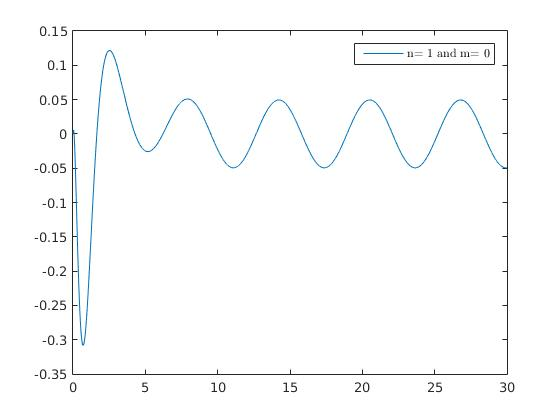
\includegraphics[width=70mm,scale=2]{assets/try10.jpg}
   \end{minipage} \hfill
    \begin{minipage}{0.48\textwidth}
  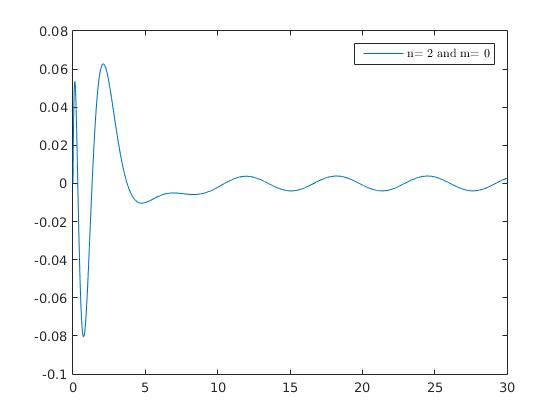
\includegraphics[width=70mm,scale=2]{assets/try20.jpg}
  \end{minipage}
\end{figure*}
 \begin{figure*}[h!]
\centering 
 	  \begin{minipage}{0.48\textwidth}
     \centering
     \advance\leftskip-2cm
  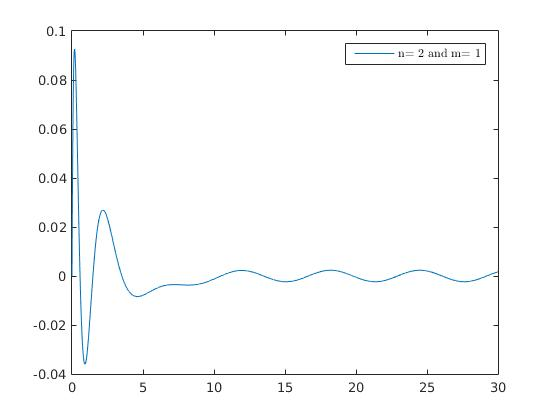
\includegraphics[width=70mm,scale=2]{assets/try21.jpg}
   \end{minipage} \hfill
    \begin{minipage}{0.48\textwidth}
  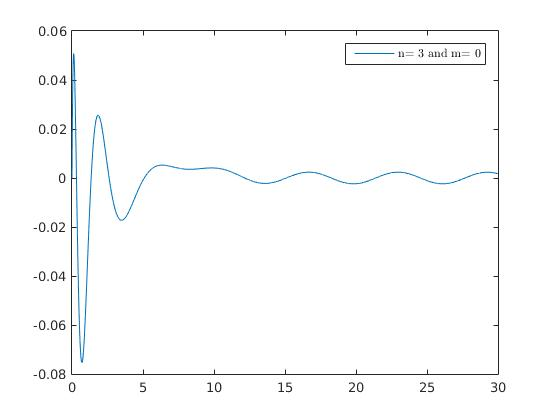
\includegraphics[width=70mm,scale=2]{assets/try30.jpg}
  \end{minipage}
\end{figure*}

 \begin{figure*}[h!]
\centering 
 	  \begin{minipage}{0.48\textwidth}
     \centering
     \advance\leftskip-2cm
  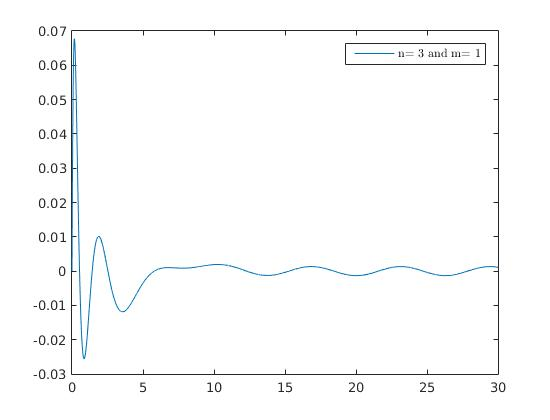
\includegraphics[width=70mm,scale=2]{assets/try31.jpg}
   \end{minipage} \hfill
    \begin{minipage}{0.48\textwidth}
  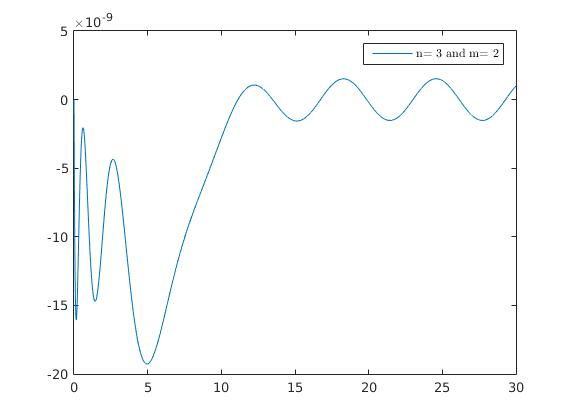
\includegraphics[width=70mm,scale=2]{assets/try32.jpg}
  \end{minipage}
\end{figure*}
\clearpage
 \begin{figure*}[h!]
\centering 
 	  \begin{minipage}{0.48\textwidth}
     \centering
     \advance\leftskip-2cm
  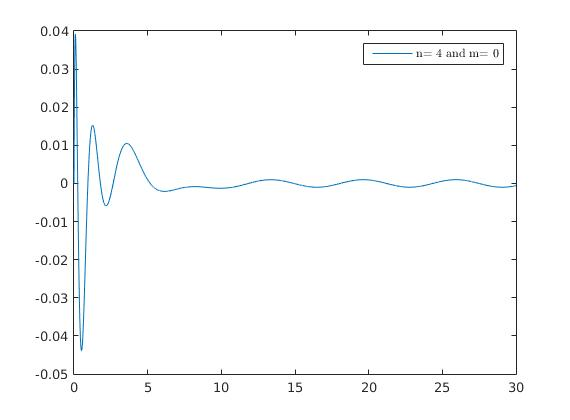
\includegraphics[width=70mm,scale=2]{assets/try40.jpg}
   \end{minipage} \hfill
    \begin{minipage}{0.48\textwidth}
  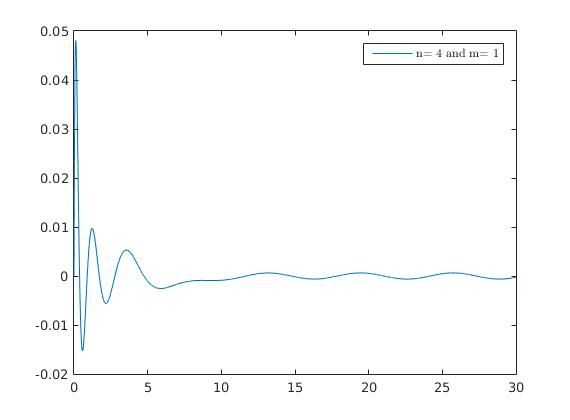
\includegraphics[width=70mm,scale=2]{assets/try41.jpg}
  \end{minipage}
\end{figure*}
 \begin{figure*}[h!]
\centering 
 	  \begin{minipage}{0.48\textwidth}
     \centering
     \advance\leftskip-2cm
  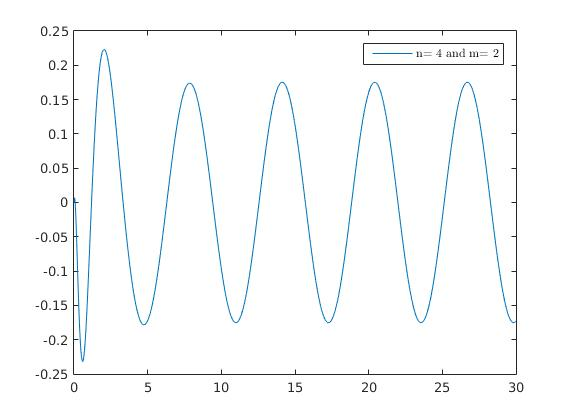
\includegraphics[width=70mm,scale=2]{assets/try42.jpg}
   \end{minipage} \hfill
    \begin{minipage}{0.48\textwidth}
  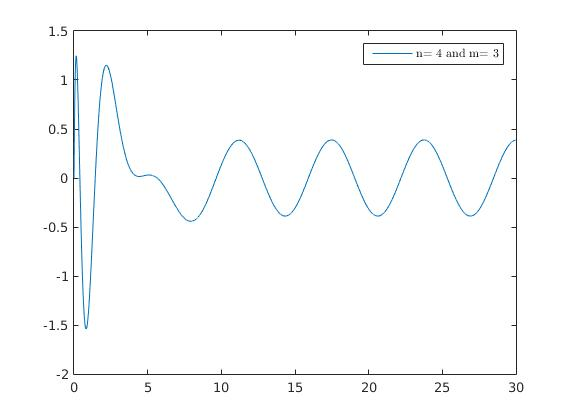
\includegraphics[width=70mm,scale=2]{assets/try43.jpg}
  \end{minipage}
\end{figure*}
Σκοπός των δοκιμών αυτών είναι να παρατηρήσουμε ποιος συνδυασμος τάξεων n και m μας οδηγεί στο μικρότερο σφάλμα και κατ επέκταση ποιο μοντελοποιημένο σύστημα προσεγγίζει καλύτερα τις τιμές εξόδου του πραγματικού. Εφόσον η επιλογή των τάξεων n και m γίνει είμαστε σε θέση να βρούμε τις τιμές των παραμέτρων του συστήματος. Ο κώδικας \textit{matlab} για την δημιουργία των παραπάνω γραφικών παραστάσεων αλλα και για τον υπολογισμό των παραμέτρων του συστήματος, υπάρχει στο αρχείο \textit{offline.m} και βρίσκεται στον φάκελο \textit{matlab\_source\_code/offline}. Στον φάκελο αυτό υπαρχουν επίσης καποια βοηθητικά αρχεία όπως:
\begin{itemize}
\item \textit{filtermaster.m}: το οποίο επιλέγει φίλτρο για το σύστημα ανάλογα με την τάξη εξόδου του συστήματος.
\item \textit{calcmaster.m}: το οποίο υπολογίζει τον πίνακα οπισθοδρομιτών φ του συστήματος.
\end{itemize}
\clearpage
\section*{Συμπέρασματα}
\Large
Δεδομένου των σφαλμάτων που παρουσιάζονται στα παραπάνω διαγράμματα, παρατηρούμε πως το μικρότερο σφάλμα της διαφοράς: \begin{center}
\textit{πραγματικής εξόδου με την εκτιμώμενη έξοδο}
\end{center}  το συναντάμε για τις τιμές\begin{center}
$\boxed{\textit{n = 3 και m = 2}}$
\end{center}
η επιλογή του φίλτρου που κάναμε για αυτή την τάξη εξόδου ήταν
\begin{center}
\textit{Λ(s) = $s^3+4s^2+5s+2$}
\end{center}
συνεπώς λαμβανοντας υπ όψιν το παραπάνω φίλτρο υπολογίζονται οι τιμές των παραμέτρων:
\begin{equation*}
{θ^{Τ}}_λ = \begin{bmatrix}
6 &  11 & 6 & 6
     &  1 & -3 & 2   
\end{bmatrix}
\end{equation*}
και το σύστημα περιγράφεται απο την διαφορική:
\begin{equation*}
y^{(3)} + 6y^{(2)} + 11\dot{y} + 6y = u^{(2)} -3\dot{u} + 2u
\end{equation*}
\par Αξίζει να σημειωθεί πως για την επιλογή των τάξεων εισόδου και εξόδου του συστήματος δεν αρκούμαστε μόνο στην παρατήρηση του σφάλματος. Σε μια περίπτωση που δύο δοκιμές (τάξης εισόδου-εξόδου) μας οδηγούσαν σε παρόμοια σφάλματα, το να στηρίζαμε την επιλογή ενός μοντέλου απλά παρατηρόντας την γραφική παράσταση με το μάτι θα ήταν αβάσιμο και επικύνδυνο. Για αυτό τον λόγο πρόκειται παρακάτω να αξιολογίσουμε τις επιλογές των τάξεων αυτων και κατ επέκταση να τεκμιριώσουμε οτι η επιλογή μας δίνει ελάχιστο σφάλμα μοντέλου.   
\large {}
\newpage
\section*{Μέθοδος πραγματικού χρόνου}
Για την εκτίμηση των παραμέτρων με μια μέθοδο πραγματικού χρόνου επιλέγουμε τον αναδρομικό αλγόριθμο ελαχίστων τετραγώνων.
\par Θεωρούμε το γραμμικά παραμετροποιημένο σύστημα:
\begin{equation*}
y = {θ^*}^Tφ
\end{equation*}
οπου y η έξοδος, ${θ^*}$ το διάνυσμα των άγνωστων αλλα σταθερών παραμέτρων και φ το διάνυσμα των οπισθιδρομητών. Τόσο η έξοδος όσο και το φ είναι μετρήσιμα. \par Έστω το σύστημα αναγνώρισης:
\begin{equation*}
\hat{y} = \hat{{θ}^T}φ 
\end{equation*}
όπου $\hat{y}$ η εκτιμώμενη έξοδος και $\hat{θ}$ το διάνυσμα των εκτιμώμενων παραμέτρων.
\par Το σφάλμα αναγνώρισης ορίζεται ως:
\begin{equation*}
\tilde{y} = y - \hat{{θ}^T}φ 
\end{equation*}
\par Θέλουμε να υπολογίσουμε την τιμή $\hat{θ}$ που θα ελαχιστοποιεί το κριτήριο:
\begin{equation*}
K(\hat{θ}) = \frac{1}{2}e^{-βt}(\hat{θ}(t) - \hat{θ}(0))^T Q_0 (\hat{θ}(t) - \hat{θ}(0)) + \frac{1}{2} \int_{0}^{t} e^{-β(t-τ)}[y(τ) - \hat{θ}(t)^Tφ(τ)]^2 dτ
\end{equation*}
οπου $Q_0$ = ${Q_0}^T$ (θετικά ορισμένος πίνακας), β$\geq$0 μια σταθερά. Η Κ($\hat{θ}$) είναι κυρτή συνάρτηση του $\hat{θ}$ . Επομένως κάθε τοπικό ελάχιστο είναι και ολικό και ικανοποιεί:
\begin{equation*}
\nabla{K(\hat{θ})} = 0
\end{equation*}
καταλήγουμε:
\begin{equation*}
\hat{θ}(t) = P(t) [ e^{-βt} Q_0 \hat{θ}(0) + \int_{0}^{t} e^{-β(t-τ)}y(τ)φ(τ) dτ]
\end{equation*}
\begin{equation*}
P(t) = [ e^{-βt} Q_0 + \int_{0}^{t} e^{-β(t-τ)}φ(τ)φ^T(τ) dτ]^{-1}
\end{equation*}
γνωρίζουμε οτι Ρ$P^{-1}$ = Ι οπου Ι ο μοναδιαίος πίνακας συνεπώς:
\begin{equation*}
\frac{d}{dt}[PP^{-1}] = 0
\end{equation*}
λύνοντας ως προς $\dot{P}$:
\begin{equation*}
\dot{P} = -P(\frac{d}{dt}P^{-1})P
\end{equation*}
\begin{equation*}
P^{-1}(t) = e^{-βt} Q_0 + \int_{0}^{t} e^{-β(t-τ)}φ(τ)φ^T(τ) dτ
\end{equation*}
\begin{equation*}
\frac{d}{dt}P^{-1} = -β P^{-1} + φφ^T
\end{equation*}
αντικαθιστώντας βγάζουμε:
\begin{equation*}
\boxed{\dot{P}=βP - Pφ φ^T P}\enspace και\enspace P(0)={Q_0}^{-1}
\end{equation*}
ομοίως:
\begin{equation*}
\hat{θ}(t) = P(t)Ω(t)
\end{equation*}
\begin{equation*}
\dot{Ω} = -βΩ +yφ \enspace Ω(0) = Q_0 \hat{θ}(0)
\end{equation*}
παραγωγίζοντας το $\hat{θ}$ καταλήγουμε:
\begin{equation*}
\boxed{
\dot{\hat{θ}} = P(t)\tilde{y}(t)φ(t)
}
\end{equation*}
\par H αναδρομική μέθοδος των ελαχίστων τετραγώνων εχει υλοποιηθεί στο αρχείο \textit{online.m}
 \par Αντίστοιχα με την offline μέθοδο πρόκειται να λύσουμε το σύστημα μέσα απο μια σειρά δοκιμών για διάφορες τιμές των n και m, παρακάτω παρουσιάζουμε τις τιμές που δοκιμάσαμε συνοπτικά στον πίνακα που ακολουθεί
\begin{center}
\begin{tabular}{ |c|c|c| } 
 \hline
$\qquad$ $\qquad$ Δοκιμές $\qquad$ $\qquad$ &$\qquad$ n $\qquad$& $\qquad$ m $\qquad$ \\ 
  \hline
 $1^{η}$ δοκιμή & 1 & 0 \\ 
  \hline
  $2^{η}$ δοκιμή & 2 & 0 \\ 
  \hline
   $3^{η}$ δοκιμή & 2 & 1 \\ 
  \hline
   $4^{η}$ δοκιμή & 3 & 0 \\ 
  \hline
   $5^{η}$ δοκιμή & 3 & 1 \\ 
  \hline
   $6^{η}$ δοκιμή & 3 & 2 \\ 
  \hline
 
\end{tabular}
\end{center}
\clearpage
\large
\begin{figure*}[h!]
\centering 
 	  \begin{minipage}{0.48\textwidth}
     \centering
     \advance\leftskip-4cm
  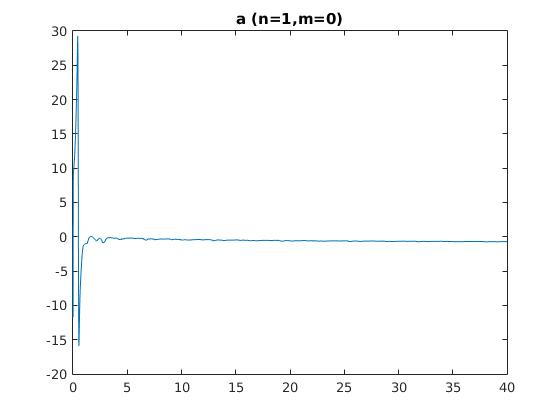
\includegraphics[width=100mm,scale=2]{assets/try10o.jpg}
   \end{minipage} \hfill
    \begin{minipage}{0.48\textwidth}
  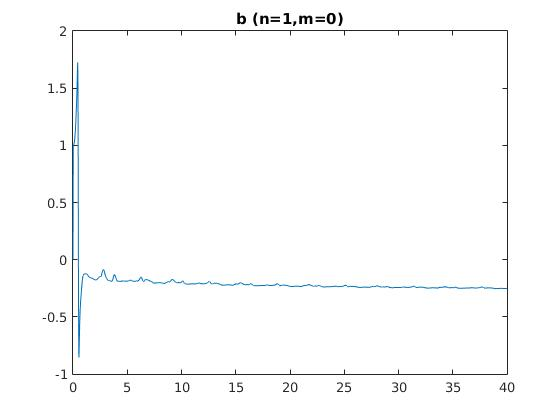
\includegraphics[width=100mm,scale=2]{assets/try10oo.jpg}
  \end{minipage}
\end{figure*}
\begin{figure*}[h!]
\centering
\advance\leftskip-0.5cm
 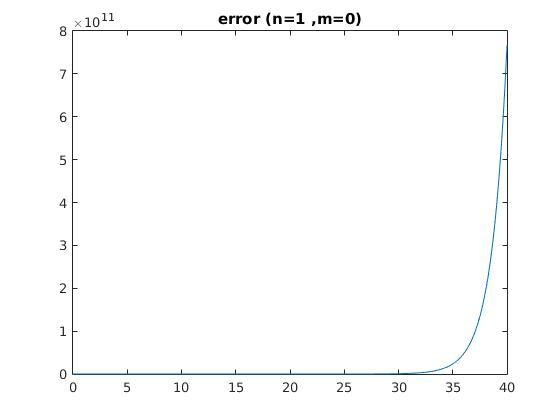
\includegraphics[width=140mm,scale=2]{assets/try10ooo.jpg}
\end{figure*}
\clearpage
\large
\begin{figure*}[h!]
\centering 
 	  \begin{minipage}{0.48\textwidth}
     \centering
     \advance\leftskip-4cm
  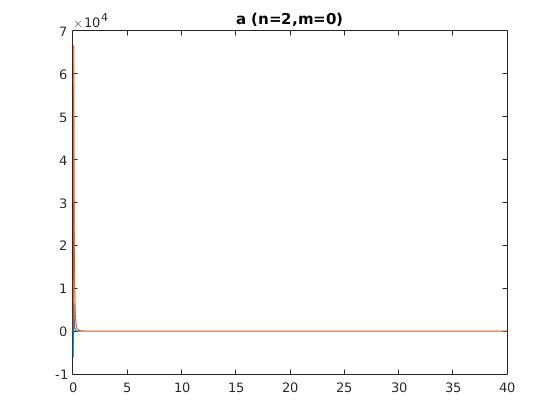
\includegraphics[width=100mm,scale=2]{assets/try20o.jpg}
   \end{minipage} \hfill
    \begin{minipage}{0.48\textwidth}
  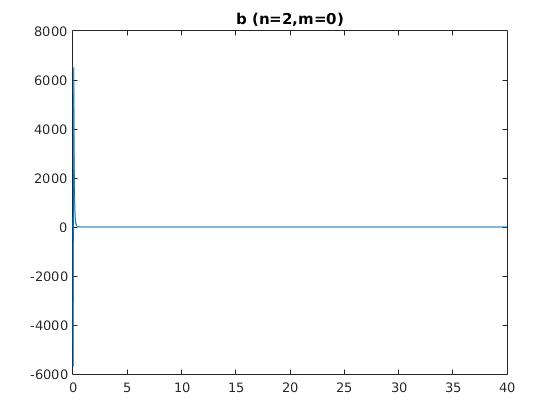
\includegraphics[width=100mm,scale=2]{assets/try20oo.jpg}
  \end{minipage}
\end{figure*}
\begin{figure*}[h!]
\centering
\advance\leftskip-0.5cm
 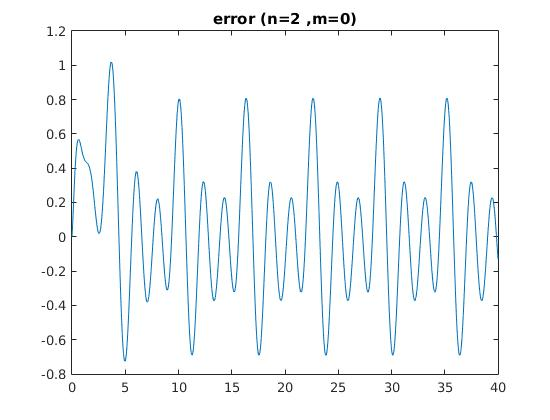
\includegraphics[width=130mm,scale=2]{assets/try20ooo.jpg}
\end{figure*}
\clearpage
\large
\begin{figure*}[h!]
\centering 
 	  \begin{minipage}{0.48\textwidth}
     \centering
     \advance\leftskip-4cm
  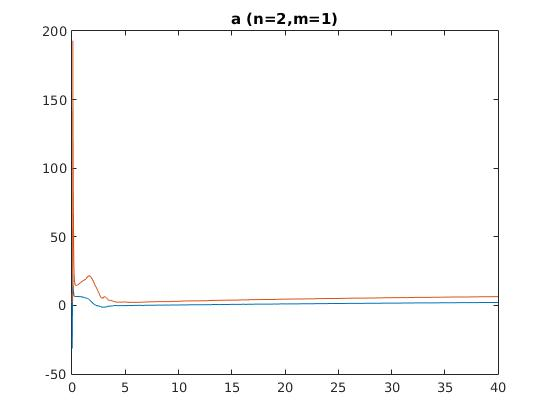
\includegraphics[width=100mm,scale=2]{assets/try21o.jpg}
   \end{minipage} \hfill
    \begin{minipage}{0.48\textwidth}
  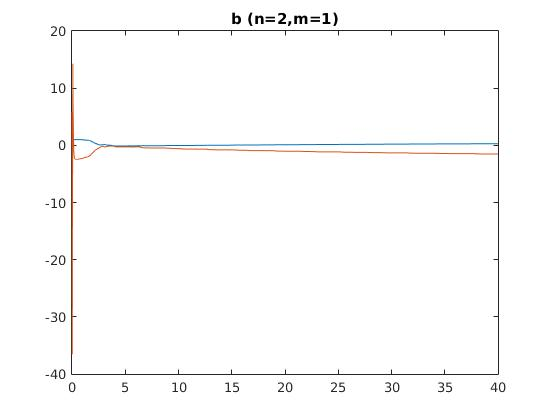
\includegraphics[width=100mm,scale=2]{assets/try21oo.jpg}
  \end{minipage}
\end{figure*}
\begin{figure*}[h!]
\centering
\advance\leftskip-0.5cm
 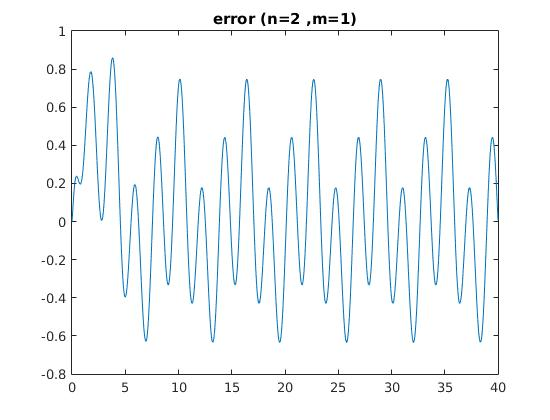
\includegraphics[width=130mm,scale=2]{assets/try21ooo.jpg}
\end{figure*}
\clearpage
\large
\begin{figure*}[h!]
\centering 
 	  \begin{minipage}{0.48\textwidth}
     \centering
     \advance\leftskip-4cm
  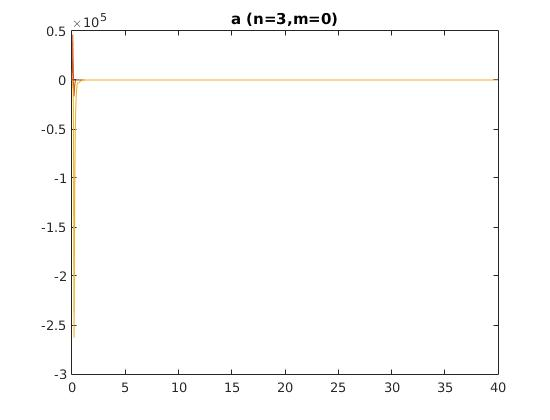
\includegraphics[width=100mm,scale=2]{assets/try30o.jpg}
   \end{minipage} \hfill
    \begin{minipage}{0.48\textwidth}
  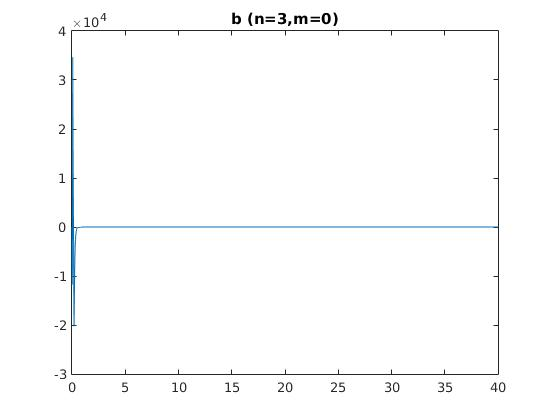
\includegraphics[width=100mm,scale=2]{assets/try30oo.jpg}
  \end{minipage}
\end{figure*}
\begin{figure*}[h!]
\centering
\advance\leftskip-0.5cm
 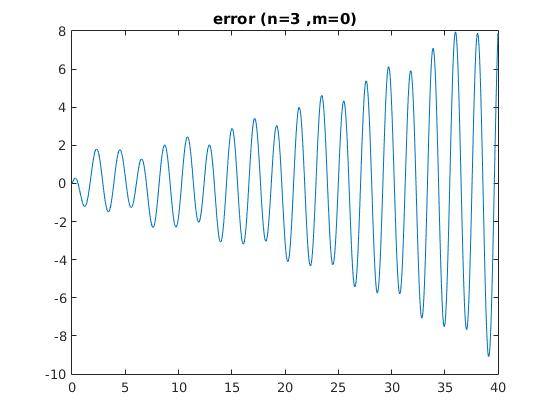
\includegraphics[width=130mm,scale=2]{assets/try30ooo.jpg}
\end{figure*}
\clearpage
\large
\begin{figure*}[h!]
\centering 
 	  \begin{minipage}{0.48\textwidth}
     \centering
     \advance\leftskip-4cm
  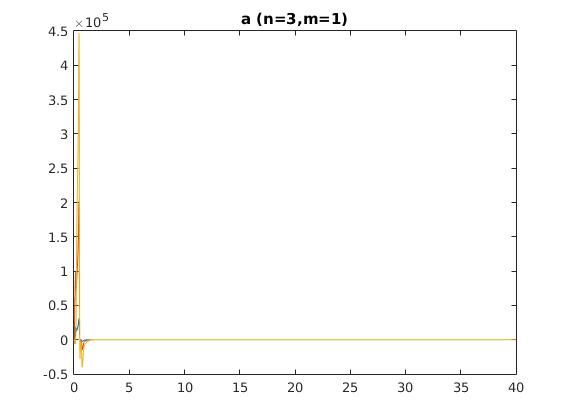
\includegraphics[width=100mm,scale=2]{assets/try31o.jpg}
   \end{minipage} \hfill
    \begin{minipage}{0.48\textwidth}
  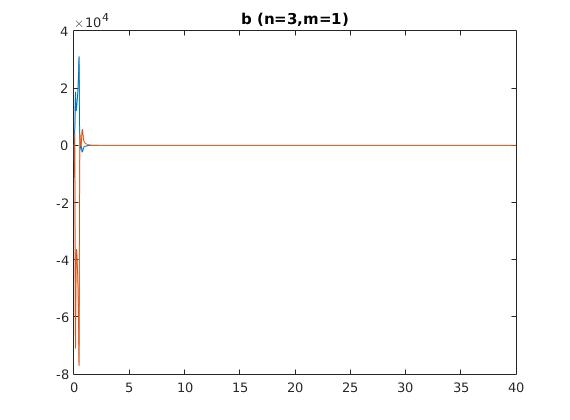
\includegraphics[width=100mm,scale=2]{assets/try31oo.jpg}
  \end{minipage}
\end{figure*}
\begin{figure*}[h!]
\centering
\advance\leftskip-0.5cm
 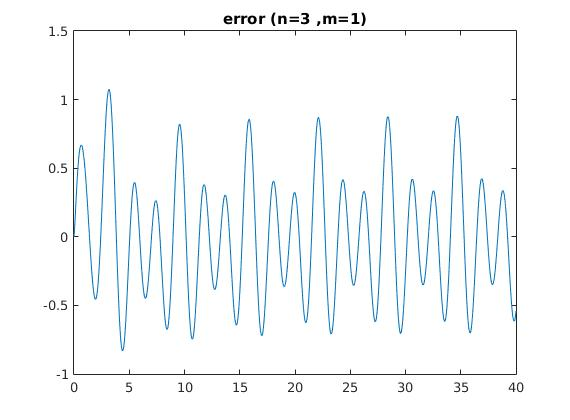
\includegraphics[width=130mm,scale=2]{assets/try31ooo.jpg}
\end{figure*}
\clearpage
\large
\begin{figure*}[h!]
\centering 
 	  \begin{minipage}{0.48\textwidth}
     \centering
     \advance\leftskip-4cm
  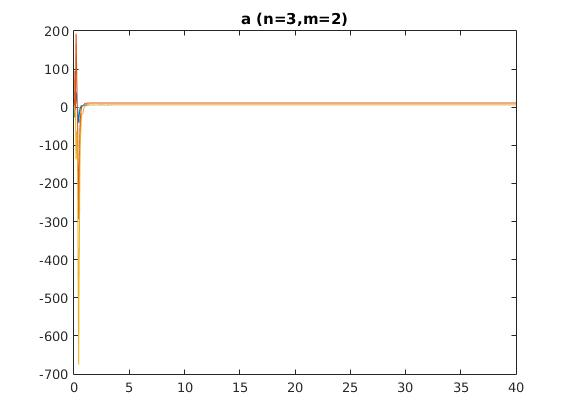
\includegraphics[width=100mm,scale=2]{assets/try32o.jpg}
   \end{minipage} \hfill
    \begin{minipage}{0.48\textwidth}
  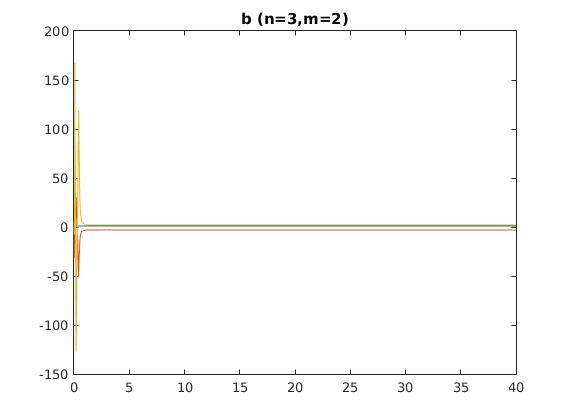
\includegraphics[width=100mm,scale=2]{assets/try32oo.jpg}
  \end{minipage}
\end{figure*}
\begin{figure*}[h!]
\centering
\advance\leftskip-0.5cm
 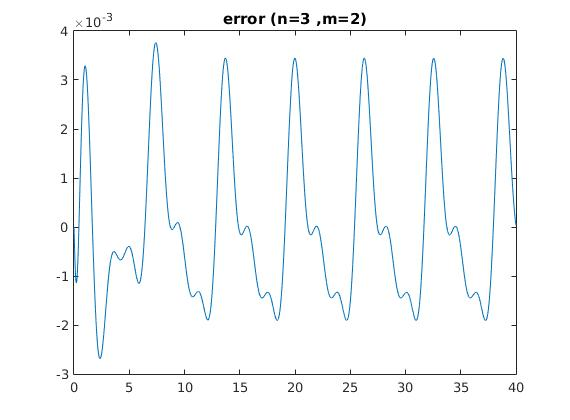
\includegraphics[width=140mm,scale=2]{assets/try32ooo.jpg}
\end{figure*}
\clearpage
\large
\begin{figure*}[h!]
\centering 
 	  \begin{minipage}{0.48\textwidth}
     \centering
     \advance\leftskip-4cm
  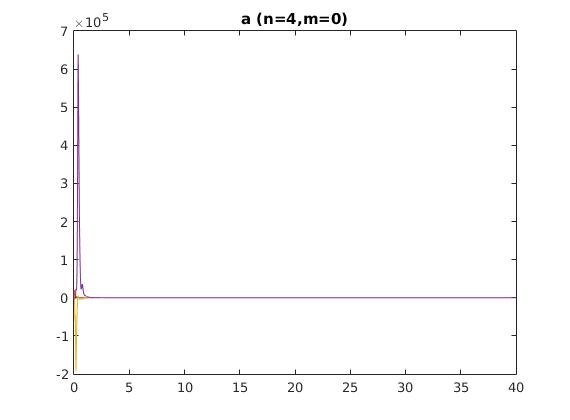
\includegraphics[width=100mm,scale=2]{assets/try40o.jpg}
   \end{minipage} \hfill
    \begin{minipage}{0.48\textwidth}
  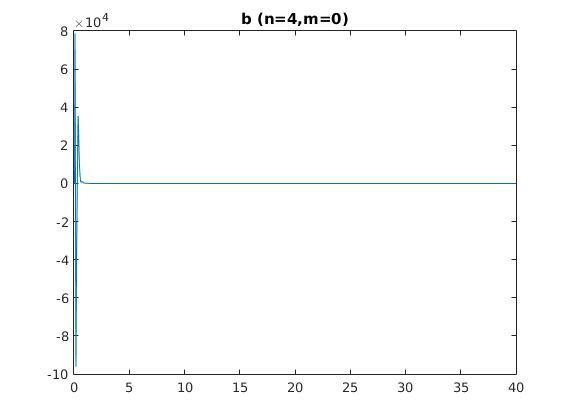
\includegraphics[width=100mm,scale=2]{assets/try40oo.jpg}
  \end{minipage}
\end{figure*}
\begin{figure*}[h!]
\centering
\advance\leftskip-0.5cm
 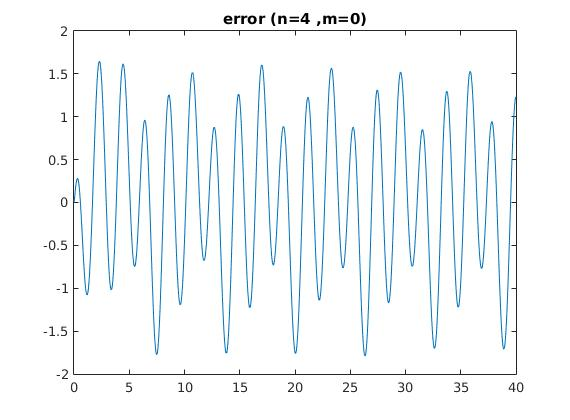
\includegraphics[width=140mm,scale=2]{assets/try40ooo.jpg}
\end{figure*}
\clearpage
\large
\begin{figure*}[h!]
\centering 
 	  \begin{minipage}{0.48\textwidth}
     \centering
     \advance\leftskip-4cm
  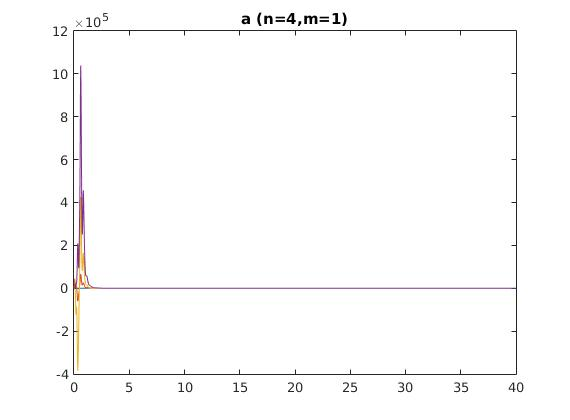
\includegraphics[width=100mm,scale=2]{assets/try41o.jpg}
   \end{minipage} \hfill
    \begin{minipage}{0.48\textwidth}
  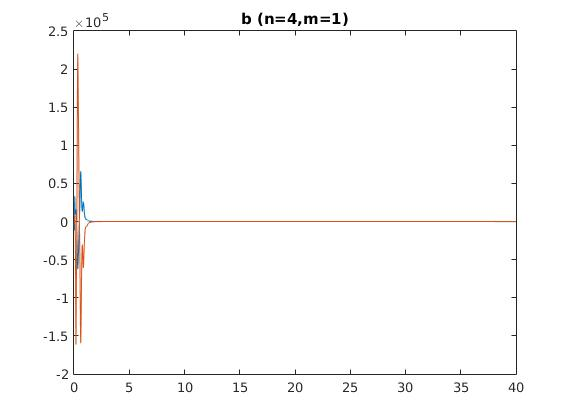
\includegraphics[width=100mm,scale=2]{assets/try41oo.jpg}
  \end{minipage}
\end{figure*}
\begin{figure*}[h!]
\centering
\advance\leftskip-0.5cm
 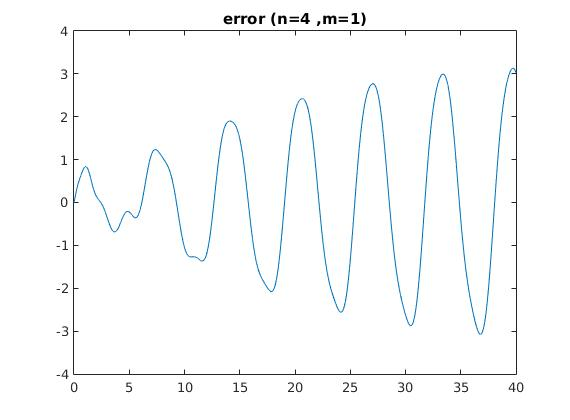
\includegraphics[width=140mm,scale=2]{assets/try41ooo.jpg}
\end{figure*}
\clearpage
\large
\begin{figure*}[h!]
\centering 
 	  \begin{minipage}{0.48\textwidth}
     \centering
     \advance\leftskip-4cm
  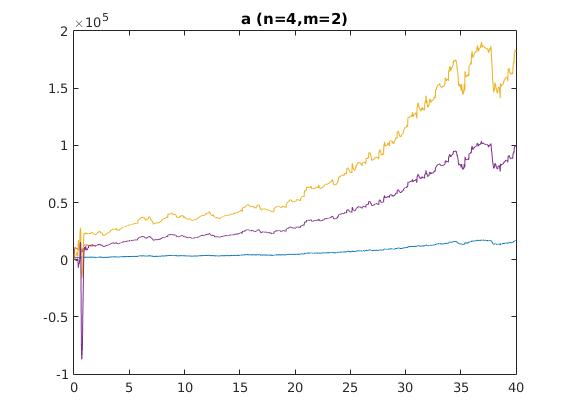
\includegraphics[width=100mm,scale=2]{assets/try42o.jpg}
   \end{minipage} \hfill
    \begin{minipage}{0.48\textwidth}
  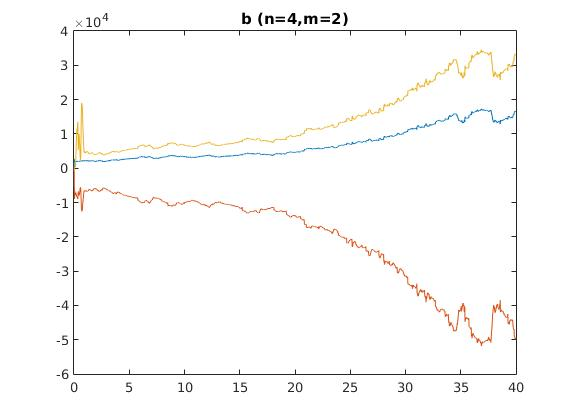
\includegraphics[width=100mm,scale=2]{assets/try42oo.jpg}
  \end{minipage}
\end{figure*}
\begin{figure*}[h!]
\centering
\advance\leftskip-0.5cm
 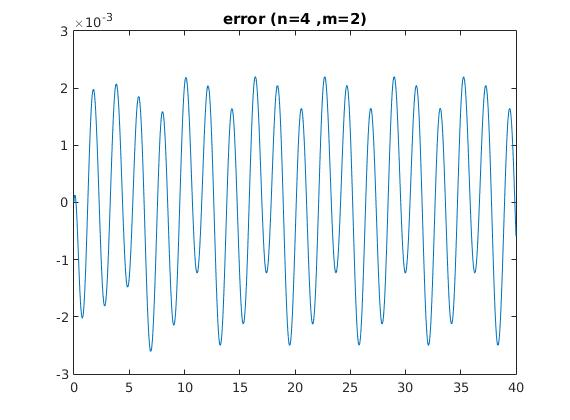
\includegraphics[width=140mm,scale=2]{assets/try42ooo.jpg}
\end{figure*}
\clearpage
\large
\begin{figure*}[h!]
\centering 
 	  \begin{minipage}{0.48\textwidth}
     \centering
     \advance\leftskip-4cm
  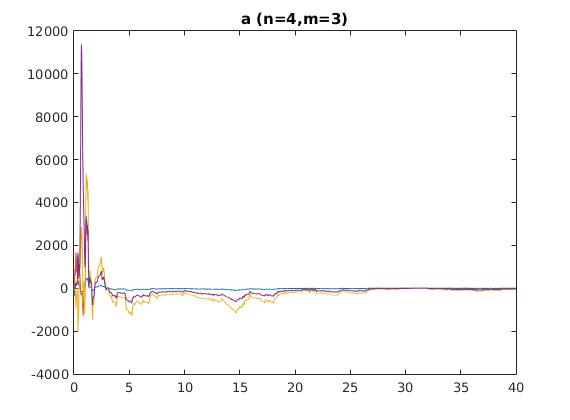
\includegraphics[width=100mm,scale=2]{assets/try43o.jpg}
   \end{minipage} \hfill
    \begin{minipage}{0.48\textwidth}
  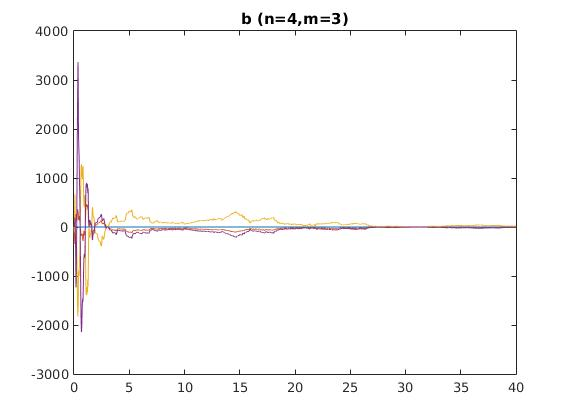
\includegraphics[width=100mm,scale=2]{assets/try43oo.jpg}
  \end{minipage}
\end{figure*}
\begin{figure*}[h!]
\centering
\advance\leftskip-0.5cm
 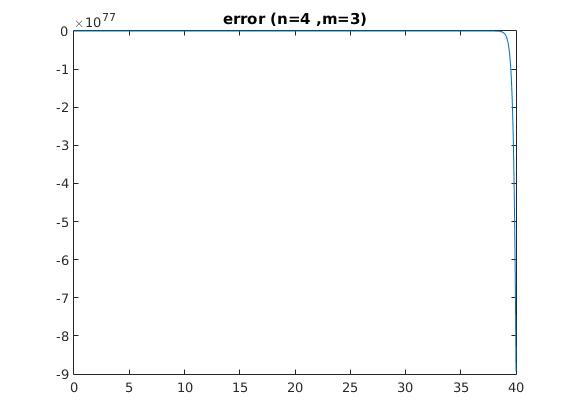
\includegraphics[width=140mm,scale=2]{assets/try43ooo.jpg}
\end{figure*}
\clearpage
 \section*{Συμπέρασματα}
 \Large{}
Δεδομένου των σφαλμάτων που παρουσιάζονται στα παραπάνω διαγράμματα, όμοια με την offline μέθοδο παρατηρούμε πως το μικρότερο σφάλμα της διαφοράς: \begin{center}
\textit{πραγματικής εξόδου με την εκτιμώμενη έξοδο}
\end{center}  το συναντάμε για τις τιμές\begin{center}
$\boxed{\textit{n = 3 και m = 2}}$
\end{center}
η επιλογή του φίλτρου ήταν ίδια με αυτη που κάναμε στην offline
\begin{center}
\textit{Λ(s) = $s^3+4s^2+5s+2$}
\end{center}
και προφανώς λαμβανοντας υπ όψιν το παραπάνω φίλτρο καταλήγουμε στις ίδιες τιμές παραμέτρων
\begin{equation*}
{θ^{Τ}}_λ = \begin{bmatrix}
6 &  11 & 6 & 6
     &  1 & -3 & 2   
\end{bmatrix}
\end{equation*}
αρα και στην ίδια διαφορική:
\begin{equation*}
y^{(3)} + 6y^{(2)} + 11\dot{y} + 6y = u^{(2)} -3\dot{u} + 2u
\end{equation*}
\\
\\
\begin{center}
\textit{ακολουθεί η αξιολόγιση των μοντέλων...}
\end{center}
 \large{}
\clearpage
\section*{Αξιολόγιση μοντέλου}
\Large
Η αξιολόγηση ενός μοντέλου μπορεί να γίνει με διάφορους τρόπους
και κριτήρια που υπάρχουν στις σημειώσεις του μαθήματος. Επιλέγουμε το κριτήριο του Akaine το οποίο περιγράφεται ως εξής:
\begin{equation*}
\boxed{AIC=Nln \left(I(θ) \right) + ρκ
}
\end{equation*}
Όπου Ν το πλήθος των δεδομένων ελέγχου, και ο αριθμός των παραμέτρων του συστήματος(n+m+1), ρ μια θετική σταθερα(επιλέχθκε ρ=2) και
\begin{equation*}
I(θ)=\frac{1}{N} \sum_{i=1}^{n} \left(y_i-\hat{y}_i \right)^{2}
\end{equation*}

\begin{center}
\begin{tabular}{ |c|c|c| } 
 \hline
$\qquad$ $\qquad$ περιπτώσεις $\qquad$ $\qquad$ &$\qquad$ ofline $\qquad$& $\qquad$ online $\qquad$ \\ 
  \hline
 μοντέλο (n=1,m=0) & 3.44$\cdot 10^6$ &  0.201$\cdot 10^7$ \\ 
  \hline
  μοντέλο (n=2,m=0) & -0.07$\cdot 10^6$ & -0.0074$\cdot 10^7$ \\ 
  \hline
 μοντέλο (n=2,m=1) & -0.09$\cdot 10^6$ & -0.0076$\cdot 10^7$ \\ 
  \hline
 μοντέλο (n=3,m=0) & 0.27$\cdot 10^6$ &  0.0095$\cdot 10^7$ \\ 
  \hline
 μοντέλο (n=3,m=1) & -0.11$\cdot 10^6$ & -0.0065$\cdot 10^7$ \\ 
  \hline
\textbf{  μοντέλο (n=3,m=2)} & -0.92$\cdot 10^6$ &   -0.0499$\cdot 10^7$ \\ 
  \hline
μοντέλο (n=4,m=0)& -0.09$\cdot 10^6$ & -0.00058$\cdot 10^7$ \\ 
  \hline
 μοντέλο (n=4,m=1) & -0.12$\cdot 10^6$ & 0.00412$\cdot 10^7$ \\ 
  \hline
 μοντέλο (n=4,m=2)& -0.79$\cdot 10^6$ & -0.0424$\cdot 10^7$ \\ 
  \hline
 μοντέλο (n=4,m=3)& 0.017$\cdot 10^6$ & 1.4122$\cdot 10^7$ \\ 
  \hline
\end{tabular}
\end{center}
   
Απο τον παραπάνω πίνακα επιβεβαιώνεται πως στην περίπτωση (n=3,m=2) εχουμε το ελάχιστο σφάλμα μοντέλου και για τις δύο μεθόδους καθώς και οτι η offline έχει μικρότερο σφάλμα μοντέλου απο την online.
\end{document}
